\documentclass[a4]{beamer}
\usepackage{amssymb}
\usepackage{graphicx}
\usepackage{subfigure}
\usepackage{newlfont}
\usepackage{amsmath,amsthm,amsfonts}
%\usepackage{beamerthemesplit}
\usepackage{pgf,pgfarrows,pgfnodes,pgfautomata,pgfheaps,pgfshade}
\usepackage{mathptmx}  % Font Family
\usepackage{helvet}   % Font Family
\usepackage{color}

\mode<presentation> {
 \usetheme{Default} % was Frankfurt
 \useinnertheme{rounded}
 \useoutertheme{infolines}
 \usefonttheme{serif}
 %\usecolortheme{wolverine}
% \usecolortheme{rose}
\usefonttheme{structurebold}
}

\setbeamercovered{dynamic}

\title[MA4413]{Statistics for Computing \\ {\normalsize Lecture 10B}}
\author[Kevin O'Brien]{Kevin O'Brien \\ {\scriptsize kevin.obrien@ul.ie}}
\date{Autumn 2013}
\institute[Maths \& Stats]{Dept. of Mathematics \& Statistics, \\ University \textit{of} Limerick}

\renewcommand{\arraystretch}{1.5}


\begin{document}
%----------------------------------------------------------------------------------------------------------%


\begin{frame}
\titlepage
\end{frame}
\begin{frame}
\frametitle{Information Theory and Source Coding}
\textbf{\textit{(Last Section of MA4413 Course)}}\\
\bigskip
\textbf{Introduction : } Information theory provides a quantitative measure of the information contained in message signal and allows us to determine the capacity of a communication system to transfer this information from source to destination. \\ \bigskip ln this part of the course, we will explore some basic ideas involved in information theory and source coding.
\end{frame}


%---------------------------------------------------------------------------------------------%
\begin{frame}
\frametitle{Introduction to Information Theory}
\begin{itemize}
\item Information theory is a process that focuses on the task of quantifying information. 
\item The quantification of information is achieved by identifying viable methods of compressing and communicating data without causing 
and degradation in the integrity of the data. 
\item Information theory can be utilized in a number of different fields, including quantum computing, 
data analysis and cryptography.
\end{itemize}
\end{frame}
%---------------------------------------------------------------------------------------------%
\begin{frame}
\frametitle{Introduction to Information Theory}
\begin{itemize}
\item The origin of modern informational theory is usually attributed to Claude E. Shannon.
\item His work A Mathematical Theory of Communication, first published in 1948, 
lays the foundation for the quantification and compression of data into viable units that may be stored for easy retrieval later. 
\item His basic approach provided the tools necessary to enhance the efficiency of early mainframe computer systems, and translated easily into 
the advent of desktop computers during the decade of the 1970’s.
\end{itemize}
\end{frame}
%---------------------------------------------------------------------------------------------%
\begin{frame}
\frametitle{Introduction to Information Theory}
\begin{itemize}

\item As a branch of both electrical engineering and applied mathematics, information theory seeks to uncover the most efficient 
methods of conveying data, within the limits inherent in the data proper. \item The idea is to ensure that the mass transit of data does 
not in any way decrease the quality, even if the data is compressed in some manner. 
\end{itemize}
\end{frame}
%---------------------------------------------------------------------------------------------%
\begin{frame}
\frametitle{Introduction to Information Theory}
\begin{itemize}
\item Ideally, the data can be restored to its original form upon reaching its destination. 
\item In some cases, however, the goal is to allow data in one form to be converted for mass transmission, 
received at the point of termination, and easily converted into a format other than the original without losing any of the transmitted information.
\end{itemize}
\end{frame}

\frame{
\frametitle{What is Information?}

\begin{itemize} \item  What is meant by the ``information" contained in an event?
\item If we are formally to defined a quantitative measure of information contained in an event, this measure should have some intuitive properties such as:
\begin{itemize} \item [1.] Information contained in events ought to be defined in terms of some measure of the uncertainty of the events.
\item [2.] Less certain events ought to contain more information than more certain events.
\item [3.] The information of unrelated / independent events taken as a single event should equal the sum of the information of the unrelated events.
\end{itemize}

\item A natural measure of the uncertainty of an event is the probability of $A$ denoted $P(A)$.
\end{itemize}
}
%----------------------------------------------------------------------------------%
%----------------------------------------------------------------------------------------------------------------------------------------------------------------------------------%


\begin{frame}
\frametitle{Measure of Information}

\textbf{1) Information sources:}\\

An information source is an object that produces an event, the outcome of which is selected at
random according to a probability distribution.  \\ \bigskip A practical source in a communication system is a
device that produces messages, and it can be either analog or discrete (we deal mainly
with the discrete sources, since analog sources can be transformed to discrete sources) \\ \bigskip A discrete information source is a
source that has only a finite set of symbols as possible outputs. The set of source symbols is called the
\textbf{\emph{source alphabet}}, and the elements of the set are called \textbf{\emph{ symbols}} or \textbf{\emph{letters}}.
\end{frame}
%----------------------------------------------------------------------------------------------------------%
\begin{frame}
\frametitle{Memory}
\begin{itemize} \item Information sources can be classified as having memory or being memoryless.
\item A source with
memory is one for which a current symbol depends on the previous symbols.\item A memoryless source is
one for which each symbol produced is independent of the previous symbols.

\item A discrete memoryless sources (DMS) can be characterized by the list of the symbols, the
probability assignment to these symbols, and the specification of the rate of generating these symbols by the source.\end{itemize}
\end{frame}

%----------------------------------------------------------------------------------------------------------%
\begin{frame}
\frametitle{Information content of a Discrete Memoryless Source}
\begin{itemize}
\item The amount of information contained in an event is closely related to its uncertainty.
\item Messages containing knowledge of high probability of occurrence convey relatively little information.

\item We note that if an event is certain (that is, the event occurs with probability of 1), then we can say that it conveys zero \textit{information}.

\item Conversely - very unlikely events are ``high information" events ( e.g. Alarms).
\end{itemize}
\end{frame}

%----------------------------------------------------------------------------------------------------------%
\begin{frame}
\frametitle{Information content of a Discrete Memoryless Source}
Thus, a mathematical measure of information should be a function of the probability of the outcome and should satisfy the following axioms:
\begin{itemize}
\item[1.] Information should be proportional to the uncertainty of an outcome.
\item[2.] Information contained in independent outcomes should add (see axioms).
\end{itemize}
\end{frame}

%----------------------------------------------------------------------------------------------------------%
\begin{frame}
\frametitle{Information Content of a Symbol}
\vspace{-1cm}
\begin{itemize}
\item Consider a DMS, denoted by X, with alphabet ${x,.x2. ...,x_n}$.
\item The information content of a symbol
$x_l$, denoted by $I(x_i)$, is defined by

\[  I(x_i)  = \mbox{log}_b\left({1 \over P(x_i)}\right) =  -\mbox{log}_b[ P(x_i) ]  \]


where $P(x_i)$ is the probability of occurrence of symbol $x_i$. \item ( We will discuss what $b$ is shortly.)
\end{itemize}
\end{frame}


%-------------------------------------------------------------------------------------------------------------------------------------------------------------------------------------------%
\begin{frame}
\frametitle{Axioms for Information theory}
Note that $I(x_i)$ satisfies the following properties;
\begin{itemize}
\item $I(x_i) = 0 $ for $P(x_i) = 1$ % i [(.r,) Z 0 for P(x() Z l (/0.2)
\item $I(x_i) \geq 0 $
\item $I(x_i) \; >\; I(x_j)$  if $P(x_i)\; < \; P(x_j)$
\item $I(x_i, x_j)  = I(x_i) + I(x_j)$ if $x_i$ and $x_j$ are independent.(This is based on laws of logarithms.)
\end{itemize}
\end{frame}











%----------------------------------------------------------------------------------------------------%
\begin{frame}
\frametitle{Units of Measurement}
\begin{itemize}
\item The unit of $I(x)$ is the bit (binary unit) if b = 2, \\ Hartley (or alternatively decit) if b = 10,\\ and nat (\emph{na}tural uni\emph{t}) if b = e (i.e. the exponential number).  \\ We will use $b = 2$. \item Here the unit bit (abbreviated ``b") is a measure of information content and is not to be confused with the term \emph{\textbf{bit}} meaning "binary digit." \item The conversion of these
units to other units can be achieved by the following relationships.
\end{itemize}

\[ \mbox{log}_2A = {\mbox{log}_e A \over \mbox{log} _e 2}   = {\mbox{log}_{10} A \over \mbox{log}_{10} 2}  \]

Remark: $ \mbox{log}_e\; A $ is also written $\mbox{ln}\; A$.
\end{frame}

%-------------------------------------------------------------------------------------------------------------------------------------------------------------------------------------------%
%  page
\begin{frame}
\frametitle{Average Information or Entropy}
\begin{itemize}
\item In a practical communication system, we usually transmit long sequences of symbols from an
information source. \item Thus, we are more interested in the average information that a source produces
than the information content of a single symbol.
\item The mean value of $ I(x_i)$ over the alphabet of source X with $n$ different symbols is given by
\[ H(X) = E[I(x_i)] = \sum^m_{i=1} P(x_i)I(x_i) \]
\[ H(X) =  - \sum^m_{i=1} P(x_i)\mbox{log}_2( P(x_i) ) \mbox{        (b/symbol)}\]
\end{itemize}
\end{frame}


%-------------------------------------------------------------------------------------------------------------------------------------------------------------------------------------------%
\begin{frame}
\frametitle{Entropy}
\begin{itemize}
\item The quantity $H(X)$ is called the \emph{\textbf{entropy}} of source $X$. \item It is a measure of the average information content per random symbol.
\item The source entropy $H(X)$ can be considered as the average amount of uncertainty
within source $X$ that is resolved by use of the alphabet.

\item Note that for if  binary source X that generates independent symbols $0$ and $1$ with equal probability, the source entropy $H(X)$ is
\[ H(X ) = -1/2 \mbox{log}_2 (1/2) - 1/2 \mbox{log}_2 (1/2) \mbox{   b/symbol}  \]
%(Remark :$\mbox{log}_2 ({1\over 2}) = -1$).
\end{itemize}
\end{frame}


%-------------------------------------------------------------------------------------------------------------------------------------------------------------------------------------------%
\begin{frame}
\frametitle{Entropy}
\begin{itemize}
\item The source entropy$ H(X)$ satisfies the following relation:
\[0 \leq H(X) \leq \mbox{log}_2(m) \]where $m$ is the size (number of symbols) of the alphabet of source X ).
\item  The lower bound corresponds to no uncertainty, which occurs when one symbol has probability $P(x_i) = l$ (i.e. X emits the same symbol all the time.
\item The upper bound corresponds to the maximum uncertainty which occurs when $P(x_i) = 1 /m$ for all $i$. that is, when all symbols are equally likely to be emitted by X.
 \end{itemize}
\end{frame}

%-----------------------------------------------------------------------------------------------------------------------------------------------------------%

\begin{frame}
\frametitle{Entropy: Example}
A DMS $X$ has four symbols $x_1 , x_2, x_3, x_4$ with probabilities $P(x_1) = 0.4, P(x_2) = 0.3. P(x_3) = 0.2.
P(x_4) = 0.1$.
\begin{itemize}
\item[(a)] Calculate $H(X)$.
\item[(b)] Find the amount of information contained in the messages $x_lx_2x_lx_3$ and $x_4x_3x_3x_2$.
\end{itemize}
\end{frame}
%-----------------------------------------------------------------------------------------------------------------------------------------------------------%

\begin{frame}
\frametitle{Entropy: Example part a}

\[ H(X) = - \sum \limits^{4}_{i=1} P(x_i) log_2 [P(x_i)] \]

\[ H(X) = -0.4\mbox{log}_2(0.4) - 0.3\mbox{log}_2(0.3)  -0.2\mbox{log}_2(0.2)  -0.1\mbox{log}_2(0.14) \]



\[ H(X) =  0.5288 + 0.5210 + 0.4644 + 0.3322  = \alert{1.85} \mbox{b/sec} \]

\end{frame}


%-----------------------------------------------------------------------------------------------------------------------------------------------------------%

\begin{frame}
\frametitle{Entropy: Example part b}
\begin{itemize}
\item (Remark: from probability, recall independent events) \bigskip
\item $P(x_lx_2x_lx_3) = 0.4\times 0.30 \times 0.40 \times 0.20  = 0.0096$ \bigskip
\item $I(x_lx_2x_lx_3) = -\mbox{log}_2(0.0096)  = 6.70$b/symbol \bigskip
\end{itemize}
\end{frame}
%-----------------------------------------------------------------------------------------------------------------------------------------------------------%

\begin{frame}
\frametitle{Entropy: Example part c}
\begin{itemize}
\item $P(x_4x_3x_3x_2) = 0.1\times 0.20 \times 0.20 \times 0.30  = 0.0012$ \bigskip
\item $I(x_lx_2x_lx_3) = -\mbox{log}_2(0.0012)  = 9.70$b/symbol \bigskip
\end{itemize}
\end{frame}


%-----------------------------------------------------------------------------------------------------------------------------------------------------------%

\begin{frame}
\frametitle{Information Rate}
If the time rate at which source X emits symbols is $r$ (symbols/second), the information rate R of the
source is given by

\[R = rH(X) \mbox{      (b/second)} \]

\end{frame}


%-----------------------------------------------------------------------------------------------------------------------------------------------------------%
\begin{frame}
\frametitle{Information Rate : Example}
\begin{itemize}

\item A high-resolution TV picture consists of about $2 \times 10^6$ picture elements (symbols) and 16
different brightness levels. \item Pictures are repeated at a rate of 32 per second. \item All picture elements
are assumed to be independent, and all levels have equal likelihood of occurrence. \item Calculate the
average rate of information conveyed by this TV picture source.

\end{itemize}
\end{frame}

%-----------------------------------------------------------------------------------------------------------------------------------------------------------%
\begin{frame}
\frametitle{Information Rate : Example}
\begin{itemize}
\item $H(X) = - \sum \limits^{16}_{i=1} {1\over16} \mbox{log}_2{1\over16}$ \bigskip

\item i.e. $H(X) = [ -{1\over16} \mbox{log}_2{1\over16} ] + [- {1\over16} \mbox{log}_2{1\over16} ] \ldots [ -{1\over16} \mbox{log}_2{1\over16}) ] $ \bigskip
\item Sixteen identical terms. Compute one and multiply by 16.

\[ H(X) = 16 \times [ -{1\over16} \mbox{log}_2{1\over16} ]  = -\mbox{log}_2{1\over16} = -(-4) = 4\] \bigskip
\item $H(X)= 4$ b
\item $r =  2(10^6)(32) = 64(10^6)$ elements/sec \bigskip

\item $R = rH(X) = 64(10^6)(4) = 256(l0^6) \mbox{ b/sec } = 256 \mbox{ Mb/sec }$ \bigskip
\end{itemize}
\end{frame}
%\end{document}
\begin{frame} \frametitle{Discrete Memoryless Channels}
%\textbf{A. Channel Representation:}\\
\begin{itemize}
\item A communication channel is the path or medium through which the symbols flow to the receiver. \item A discrete memoryless channel (DMC) is a statistical model with an input X and an output Y.
During each unit of the time, the channel accepts an input symbol from X, and in
response it generates an output symbol from Y. \item  The channel is ``discrete" when the alphabets of X and
Y are both finite.\item It is ``memoryless" when the current output depends on only the current input and
not on any of the previous inputs.\end{itemize}
\end{frame}

%--------------------------------------------------------%

\frame{
\frametitle{Discrete Memoryless Channels}

\begin{center}
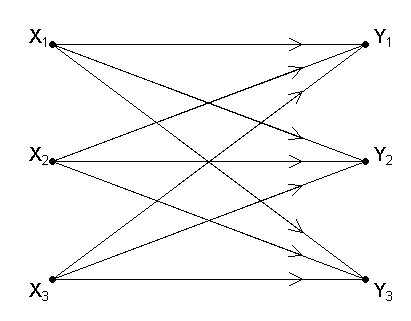
\includegraphics[scale=0.54]{10Bnet}
\end{center}

}


%\end{document}
\begin{frame}
\frametitle{Discrete memoryless channel}
\begin{itemize}
\item A DMC can have any number of inputs and any number of outputs.
\item For a DMC with ``m" inputs and ``n" outputs, the input X consists of input symbols $x_1, x_2, \ldots x_m$.
\item The probabilities of these source symbols $P(x_i)$ are assumed to be known.
\item The output Y consists of output symbols $\{y_1,y_2,\ldots, y_n \}$
\item Each possible input-to-output path is indicated along with a conditional probability $P(y_i|x_i)$, where $P(y_i|x_i)$  is the conditional probability of
obtaining output $y_i$ given that the input is $x_i$. \item $P(y_i|x_i)$ is called a \textbf{\emph{channel transition probability}}.
\end{itemize}
\end{frame}
%\end{document}
%--------------------------------------------------------%
%--------------------------------------------------------%
\begin{frame}
\frametitle{Discrete memoryless channel}
\begin{itemize}
\item On the next slide, we present a binary DMC, with the channel transition probabilities indicated.
\item $P(Y_1|X_1)$ = 0.9  and $P(Y_2|X_1)$ = 0.1
\item $P(Y_1|X_2)$ = 0.2  and $P(Y_2|X_2)$ = 0.8
\end{itemize}
\end{frame}

\frame{
\frametitle{Discrete Memoryless Channels}

\begin{center}
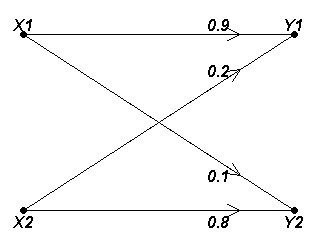
\includegraphics[scale=0.54]{10Bnet2}
\end{center}

}

%\frame{
%\frametitle{Discrete Memoryless Channels}
%
%\begin{center}
%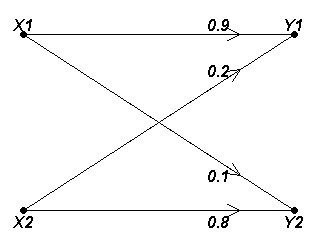
\includegraphics[scale=0.54]{10Bnet2}
%\end{center}
%}
%- Data Compression ( www.datacompression.com )

\begin{frame}
\frametitle{Channel Matrix}

A channel is completely specified by the complete set of transition probabilities. Accordingly, a
channel is specified by the matrix of transition probabilities $[P(YlX)]$, given by

\[  [P(Y|X)]  = \left[ \begin{array}{cccc}
P(y_1|x_1) & P(y_2|x_1) & \ldots & P(y_n|x_1) \\
P(y_1|x_2) & P(y_2|x_2) & \ldots & P(y_n|x_2) \\
\ldots & \ldots & \ldots & \ldots \\
P(y_1|x_m) & P(y_2|x_m) & \ldots & P(y_n|x_n) \\
\end{array} \right] \]


The matrix $[P(YlX)]$ is called the \textbf{\emph{channel matrix}}.
%ZP(yylx;) : l lor all 1 (10.12)
 \end{frame}

\begin{frame}
\frametitle{Channel Matrix}
\begin{itemize}
\item Since each input to the channel results in some
output, each row of the channel matrix must sum to unity (i.e. all rows must add up to 1. This condition is not necessary for columns).
\item For the binary DMC presented previously, the channel matrix is
\[  [P(Y|X)]  = \left[ \begin{array}{cc}
0.9 & 0.1  \\
0.2 & 0.8 \\
\end{array} \right] \]
\item (Remark: This is not a binary symmetric channel)
\end{itemize}
\end{frame}


\begin{frame}
\frametitle{Channel Matrix}
\begin{itemize}
\item The input probabilities $P(X)$ are represented by the row matrix
\[  [P(X)]  = \left[ \begin{array}{cccc}
P(x_1) & P(x_2) & \ldots & P(x_m) \\
\end{array} \right] \]
\item The input probabilities $P(Y)$ are represented by the row matrix
\[  [P(Y)]  = \left[ \begin{array}{cccc}
P(y_1) & P(y_2) & \ldots & P(y_n) \\
\end{array} \right] \]
\item We can compute $[P(Y)] $ by the following formula: $[P(Y)]  = [P(X)]\times [P(Y|X)]$
\item (Note: Be mindful of the dimensions of each matrix).
\end{itemize}
\end{frame}

\begin{frame}
\frametitle{Channel Matrix}
\begin{itemize}
\item Suppose for our Binary DMC that the input probabilities were given by $[P(X)] = [ 0.5\mbox{   }0.5]$.
\item Compute $[P(Y)]$, given the channel matrix given in previous slides.
\[  [P(Y)]  =  \left[ \begin{array}{cc}
0.5 & 0.5 \\
\end{array} \right] \times \left[ \begin{array}{cc}
0.9 & 0.1  \\
0.2 & 0.8 \\
\end{array} \right] \]

\item Solving
\[  [P(Y)]  =  \left[ \begin{array}{cc}
(0.5 \times 0.9)+(0.5 \times 0.2) & (0.5 \times 0.1)+(0.5 \times 0.8) \\
\end{array} \right]  \]

\item Simplifying \[  [P(Y)]  =  \left[ \begin{array}{cc}
0.55 & 0.45 \\
\end{array} \right]  \]
\end{itemize}
\end{frame}


\begin{frame}
\frametitle{Channel Matrix}
\begin{itemize}
\item Let $[P(X)]$ is presented as a diagonal matrix , i.e.

\[  [P(X)]_d  = \left[ \begin{array}{cccc}
P(x_1) &0 & \ldots & 0 \\
0 & P(x_2)& \ldots & 0 \\
\ldots & \ldots & \ldots & \ldots \\
0& 0 & \ldots & P(x_m) \\
\end{array} \right] \]
\item The \emph{\textbf{ joint probability matrix}} $[P(X,Y)]$can be computed as
$[P(X,Y)]  = [P(X)]_d\times [P(Y|X)]$
\end{itemize}
\end{frame}

\begin{frame}
\frametitle{Channel Matrix}
\begin{itemize}
\item For the Binary DMC described in the previous example, compute the joint probability matrix.
\item Diagonalize the input probabilities for $X$.
\[  [P(X)]_d  = \left[ \begin{array}{cc}
0.5 & 0.0  \\
0.0 & 0.5\\
\end{array} \right] \]

\item Simplifying
\[  [P(X,Y)]  =  \left[ \begin{array}{cc}
(0.5 \times 0.9)+(0 \times 0.2) & (0.5 \times 0.1)+(0 \times 0.8) \\
(0 \times 0.9)+(0.5 \times 0.2) & (0 \times 0.1)+(0.5 \times 0.8) \\
\end{array} \right]  \]


\item Solving
\[  [P(X,Y)]  =  \left[ \begin{array}{cc}
0.45 & 0.05 \\
0.1  & 0.4 \\
\end{array} \right]  \]
\end{itemize}
Notice the row and column totals.
\end{frame}
\end{document}
%---------------------------------------------------------------------------------------------------------------------------------------------------%
